\documentclass[a4paper,11pt]{report}

\usepackage[T1]{fontenc}
\usepackage[utf8]{inputenc}
\usepackage{lmodern}
\usepackage[francais]{babel}
\usepackage{graphicx}

\title{Des réseaux et des drônes}
\author{Olivier \bsc{Boissard}, Kevin \bsc{Boulala}}
\date{}

\begin{document}
\maketitle
\tableofcontents

\chapter{Les drônes}
\section{Définition}
Un drone correspond normalement à un appareil sans pilote militaire, mais il est utilisé aujourd'hui dans un sens bien plus large pour tout appareil volant sans pilote (normalement appelé aéronef). Ici, nous parlerons d'appareil volant sans pilote. Les drones peuvent avoir plusieurs formes selon leur utilisation, mais il y en a 2 principales :
\begin{itemize}
  \item avec hélice ou rotors (souvent 4 ou plus)
  \item une forme d'avion
\end{itemize}
Ils peuvent faire quelques dizaines de centimètres d'envirgures jusqu'à plusieurs dizaines de mètres (exemple : le Global Hawk fait 40 mètres d'envergure).

\section{À quoi ça sert ?}
Comme très souvent, l'idée d'origine était d'utiliser des appareils volants sans pilote à des fins militaires : la surveillance, des attaques risquées, entraîner les pilotes, réaliser des missions à plusieurs heures de vols (un pilote tenant environ 2H en vol, un drône selon sa conception peut tenir plus de 40H)...

Pour le civil, les utilisations sont multiples mais elles sont l'extension de choses qu'on pouvait faire avant avec difficulté ou très coûteuses comme les prises de vues aériennes, le transport de documents, ou pour la recherche : accéder à des zones dangereuses et/ou difficiles d'accès.

Mais les drones ont apporté de nouvelles utilisations notamment pour les réseaux informatiques.

\chapter{L'utilisation des drones pour créer un réseau informatique}
\section{Facebook et les drones lasers}
\begin{flushleft}
\includegraphics[width=\textwidth]{../Images/facebook_aquila.png}
\end{flushleft}
L'Aquila de Facebook : une grande aile de fibre de carbone d'environ 47 mètres d'envergure faisant moins 450kg. Placé par montgolfière, à une altitude oscillant entre 18 et 27km, puis elle utilisera 4 moteurs à hélices. Les drônes comminqueront via des lasers entre eux, mais aussi avec des équipements de communication au sol

Intérêts :
\begin{itemize}
  \item Connecter les zones où la population n'a pas encore d'accès à internet (soit environ 10\% de la population totale)
  \item En cas de catastrophe naturel, ce serait une solution relativement peu chère et rapide d'installation pour reconnecter ces zones
\end{itemize}

Problèmes :
\begin{itemize}
  \item Une autonomie de 3 mois. Qu'est-ce qui se passe une fois les batteries vides ?
\end{itemize}
\includegraphics[width=\textwidth]{../Images/schema_aquila.png}

\end{document}
